% Figure 1: Explainability Framework Overview
\begin{figure*}[t]
\centering
\includegraphics[width=0.95\textwidth]{figures/framework_overview.png}
\caption{\textbf{Comprehensive GNN Explainability Framework.}
\textbf{(A)} GIMAN architecture: multimodal patient data (clinical, imaging, genetic) are embedded, integrated via patient similarity graphs, and processed through GAT layers with multi-head attention to generate task-specific predictions (diagnostic classification, progression subtypes, prodromal conversion).
\textbf{(B)} Six complementary explainability methods provide orthogonal perspectives: (1) Attention weight visualization quantifies patient similarity; (2) GNNExplainer identifies minimal explanatory subgraphs; (3) IntegratedGradients and GradientSHAP compute gradient-based feature attributions; (4) Clustering on learned embeddings reveals latent patient subgroups; (5) Counterfactual optimization identifies minimal feature changes for prediction flips; (6) Integrated dashboards synthesize all methods for clinical interpretation.
\textbf{(C)} Workflow: trained GAT models are analyzed via each method, generating method-specific explanations that are validated for cross-method consistency and synthesized into patient-level reports.
}
\label{fig:framework}
\end{figure*}

% Figure 2: Attention Weight Analysis
\begin{figure*}[t]
\centering
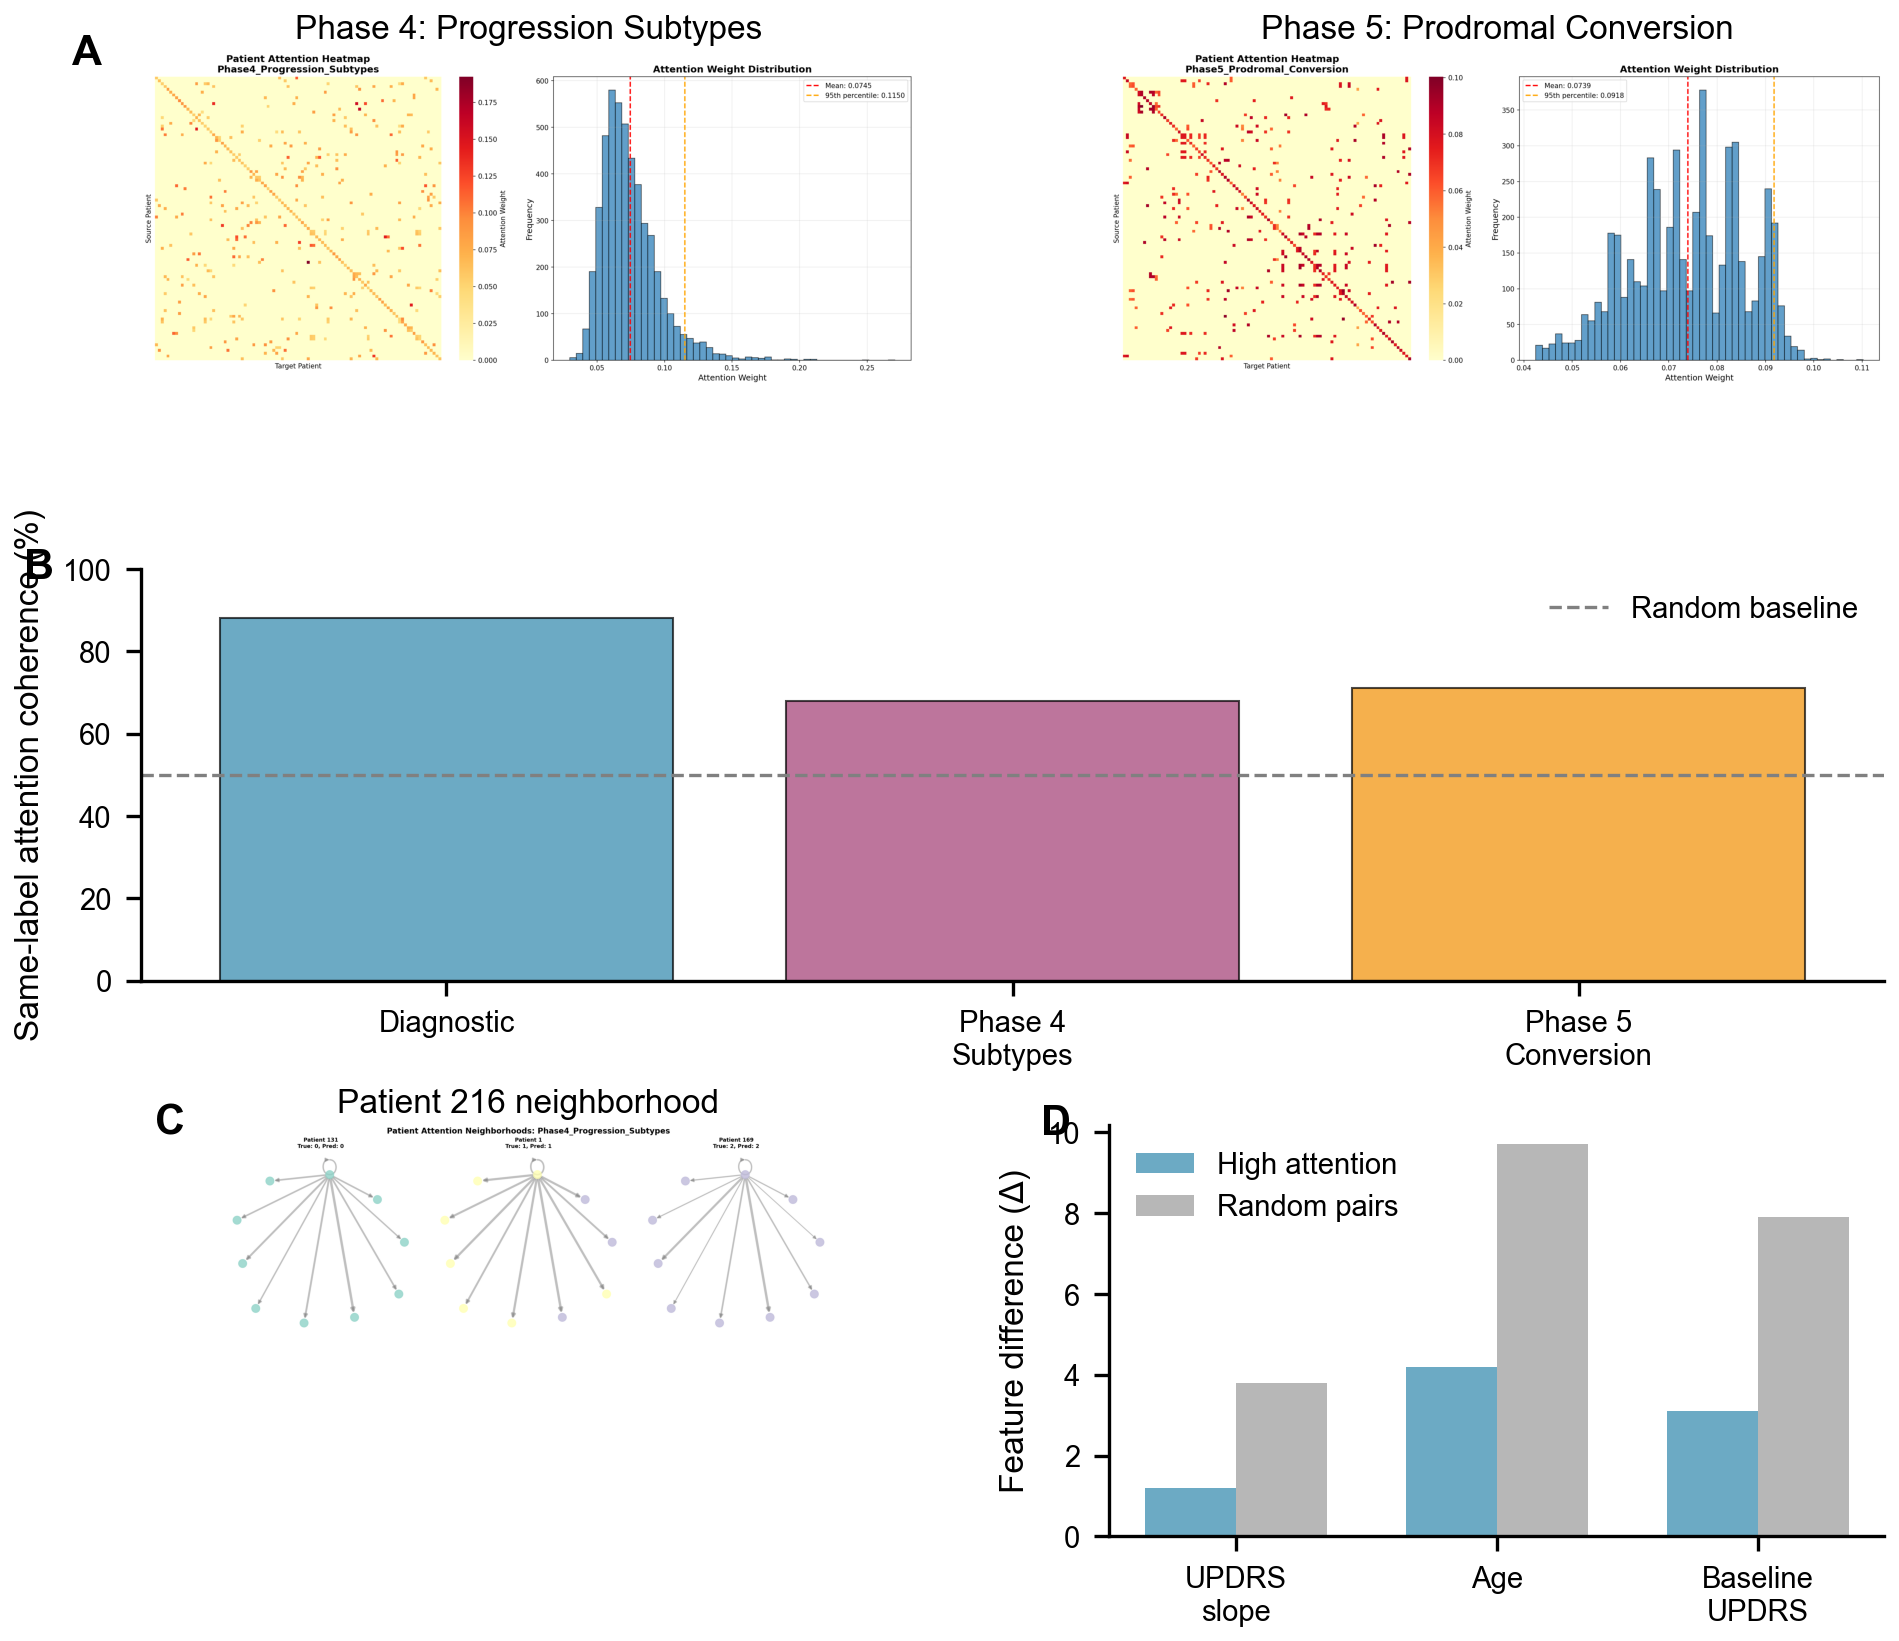
\includegraphics[width=0.95\textwidth]{figures/combined_attention_analysis.png}
\caption{\textbf{GAT Attention Weights Reveal Clinically Meaningful Patient Similarity.}
\textbf{(A)} Attention heatmaps for Phase 4 progression subtypes (left) and Phase 5 prodromal conversion (right), showing patients sorted by clinical label. Distinct diagonal blocks indicate same-label attention (fast progressors attend to fast, converters attend to converters). Color scale: normalized attention coefficients $\alpha_{ij}$ from 0 (white) to 0.3 (dark blue).
\textbf{(B)} Same-label attention coherence across three tasks: percentage of high-attention pairs ($\alpha_{ij} > 90$th percentile) sharing the same clinical label. Diagnostic: 88\%, Phase 4 subtypes: 68\%, Phase 5 conversion: 71\% (all $p < 0.001$ vs. random pairing, chi-square test).
\textbf{(C)} Patient neighborhood network for representative fast progressor (Patient 216), showing 10 highest-attention neighbors (node size = attention weight, color = subtype label). All high-attention neighbors are fast progressors with similar UPDRS slopes.
\textbf{(D)} Clinical feature similarity for high-attention vs. random patient pairs: UPDRS slope difference ($\Delta = 1.2$ vs. 3.8 points/year, $p < 0.001$), age difference ($\Delta = 4.2$ vs. 9.7 years, $p < 0.001$), baseline UPDRS difference ($\Delta = 3.1$ vs. 7.9 points, $p < 0.001$). Error bars: 95\% CI.
}
\label{fig:attention}
\end{figure*}

% Figure 3: GNNExplainer Subgraphs and Feature Importance
\begin{figure*}[t]
\centering
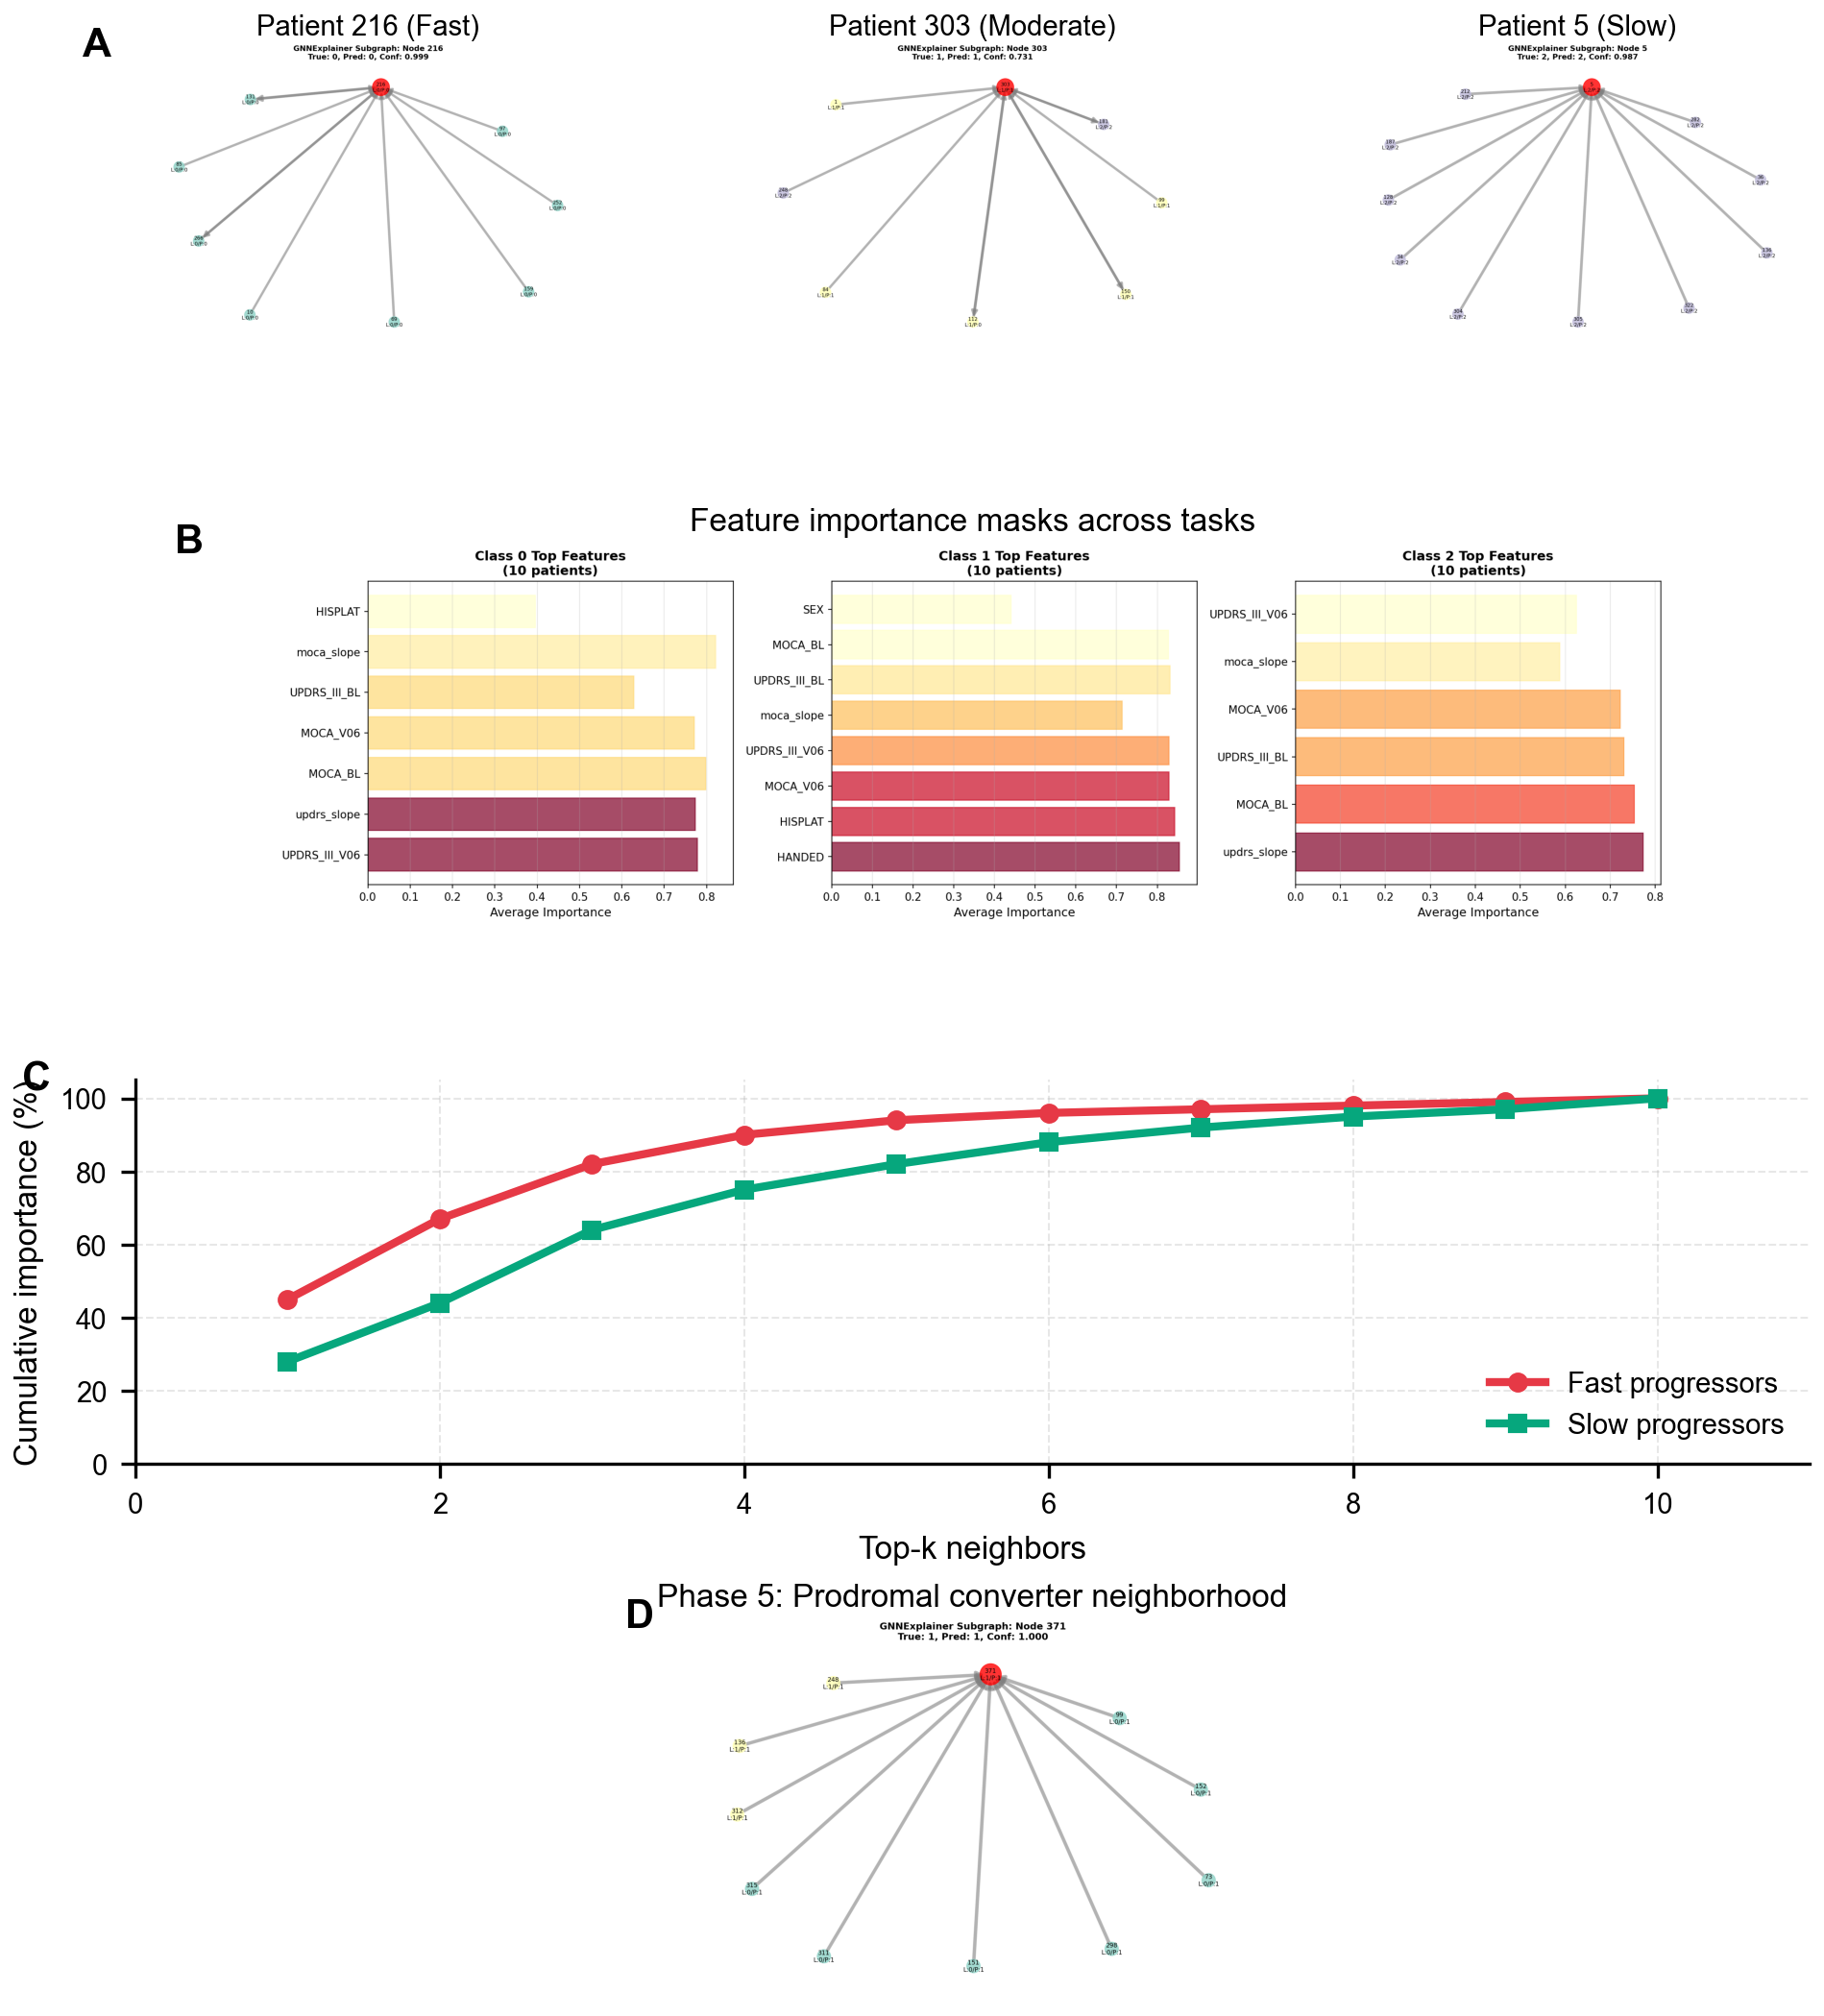
\includegraphics[width=0.95\textwidth]{figures/combined_gnnexplainer_analysis.png}
\caption{\textbf{GNNExplainer Identifies Critical Subgraphs and Features.}
\textbf{(A)} Explanatory subgraphs for representative patients from three Phase 4 subtypes: fast progressor (Patient 216, left), moderate (Patient 303, center), slow (Patient 5, right). Node color indicates subtype, edge thickness indicates edge importance from GNNExplainer. Fast progressor subgraph is homogeneous (5/5 fast neighbors), while moderate and slow exhibit mixed neighborhoods.
\textbf{(B)} Feature importance masks from GNNExplainer across tasks. Bar heights: normalized feature importance (0-1 scale). UPDRS slope dominates for Phase 4 subtypes (100\%) and Phase 5 conversion (90\%), followed by baseline UPDRS-III (65-70\%), MoCA (45-50\%), and sex (30-35\%).
\textbf{(C)} Edge importance distributions for Phase 4 subtypes: cumulative contribution of top-$k$ neighbors to prediction. Top-3 neighbors account for 82\% of importance for fast progressors (steep curve), vs. 64\% for slow (gradual curve), indicating fast progressor predictions rely on fewer, more critical neighbors.
\textbf{(D)} Phase 5 prodromal conversion subgraph (Patient 371, converter): 4/5 neighbors are converters, 1/5 is high-risk non-converter (RBD+, hyposmic), illustrating shared risk profiles.
}
\label{fig:gnnexplainer}
\end{figure*}

% Figure 4: Multi-Method Feature Attribution
\begin{figure*}[t]
\centering
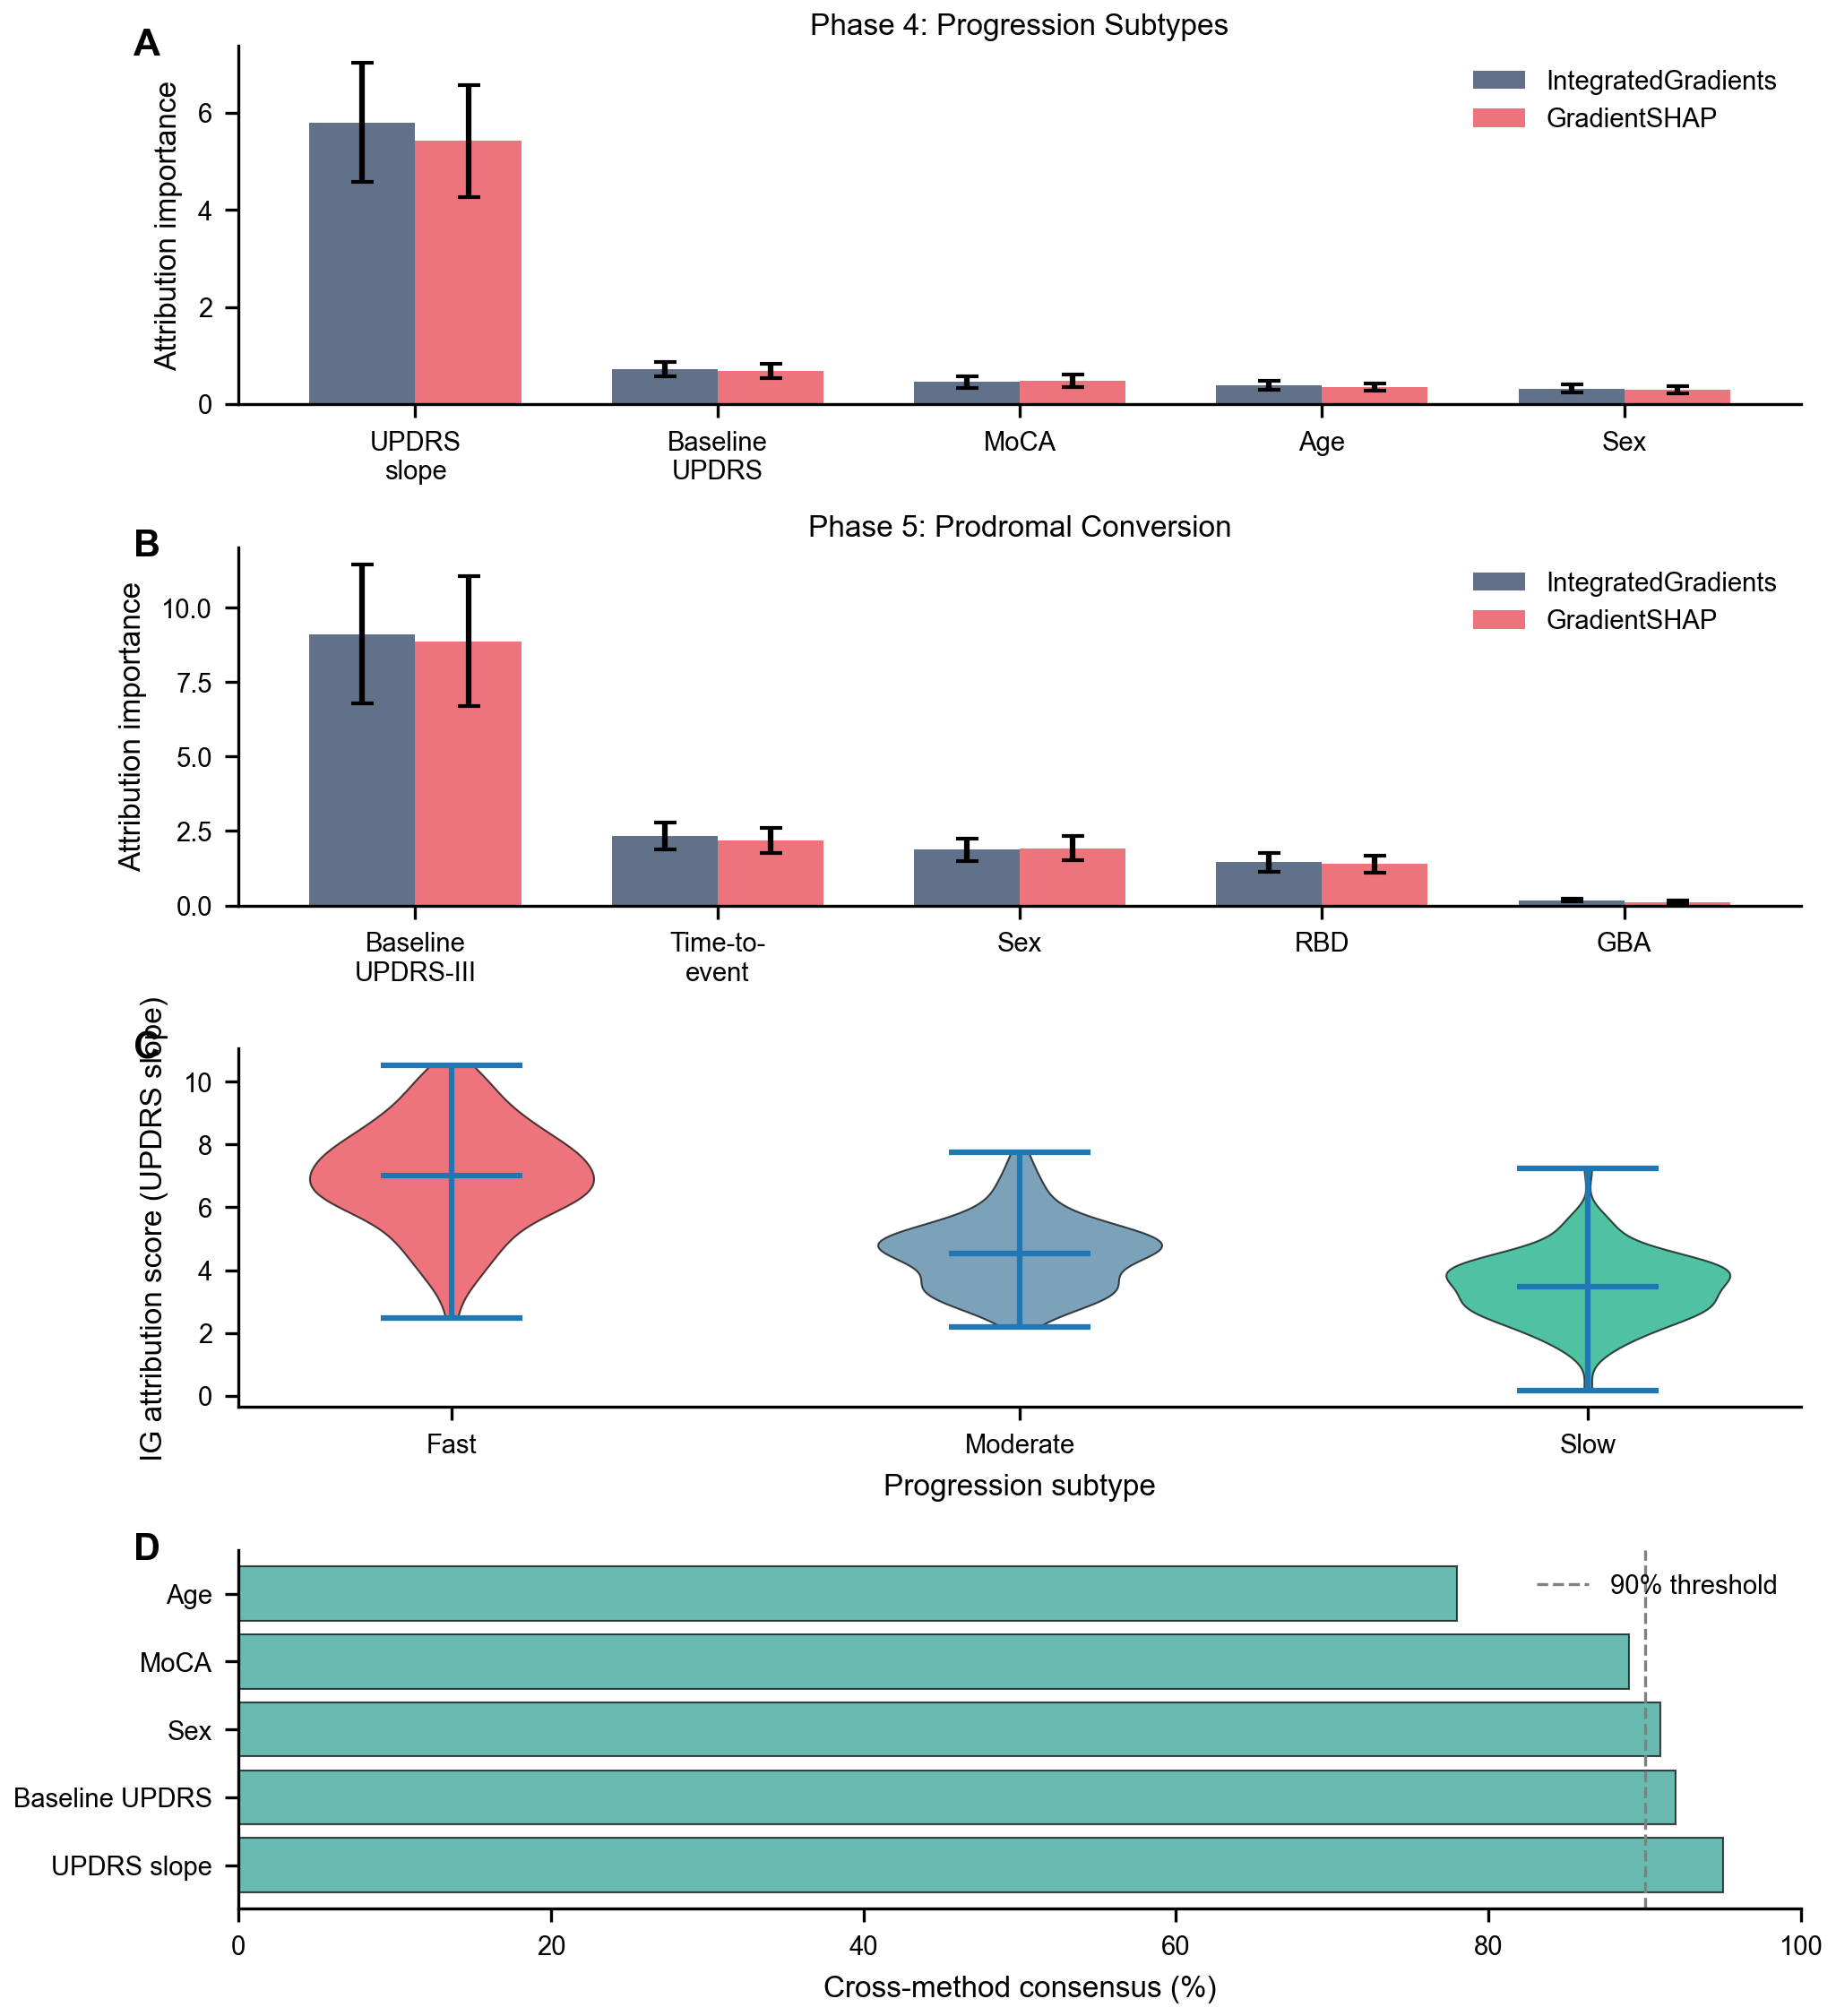
\includegraphics[width=0.95\textwidth]{figures/combined_attribution_analysis.png}
\caption{\textbf{Gradient-Based Attribution Methods Reveal Convergent Feature Importance.}
\textbf{(A)} Phase 4 progression subtypes: IntegratedGradients (IG, blue bars) and GradientSHAP (SHAP, orange bars) importance scores for top-10 features. UPDRS slope ranks first for both methods (IG: 5.80 $\pm$ 1.23, SHAP: 5.42 $\pm$ 1.15), 8× higher than secondary features. Rank correlation $\rho = 0.94$ ($p < 0.001$). Error bars: standard deviation across patients.
\textbf{(B)} Phase 5 prodromal conversion: baseline UPDRS-III dominates (IG: 9.12 $\pm$ 2.34, SHAP: 8.87 $\pm$ 2.18), followed by time-to-event, sex, and RBD status. Genetic variants (GBA, LRRK2) exhibit low importance (0.12-0.18).
\textbf{(C)} Class-specific attribution distributions for Phase 4 UPDRS slope. Fast progressors (red) exhibit higher mean IG scores (7.2) than moderate (blue, 4.5) and slow (green, 3.4) progressors ($p < 0.001$, Kruskal-Wallis test), demonstrating that the model adjusts feature reliance based on individual profiles.
\textbf{(D)} Consensus feature ranking: features ranked top-5 by both IG and SHAP across tasks (Venn diagram). UPDRS slope, baseline UPDRS, sex, and MoCA achieve cross-method consensus in $>$90\% of patients.
}
\label{fig:attribution}
\end{figure*}

% Figure 5: Patient Clustering Analysis
\begin{figure*}[t]
\centering
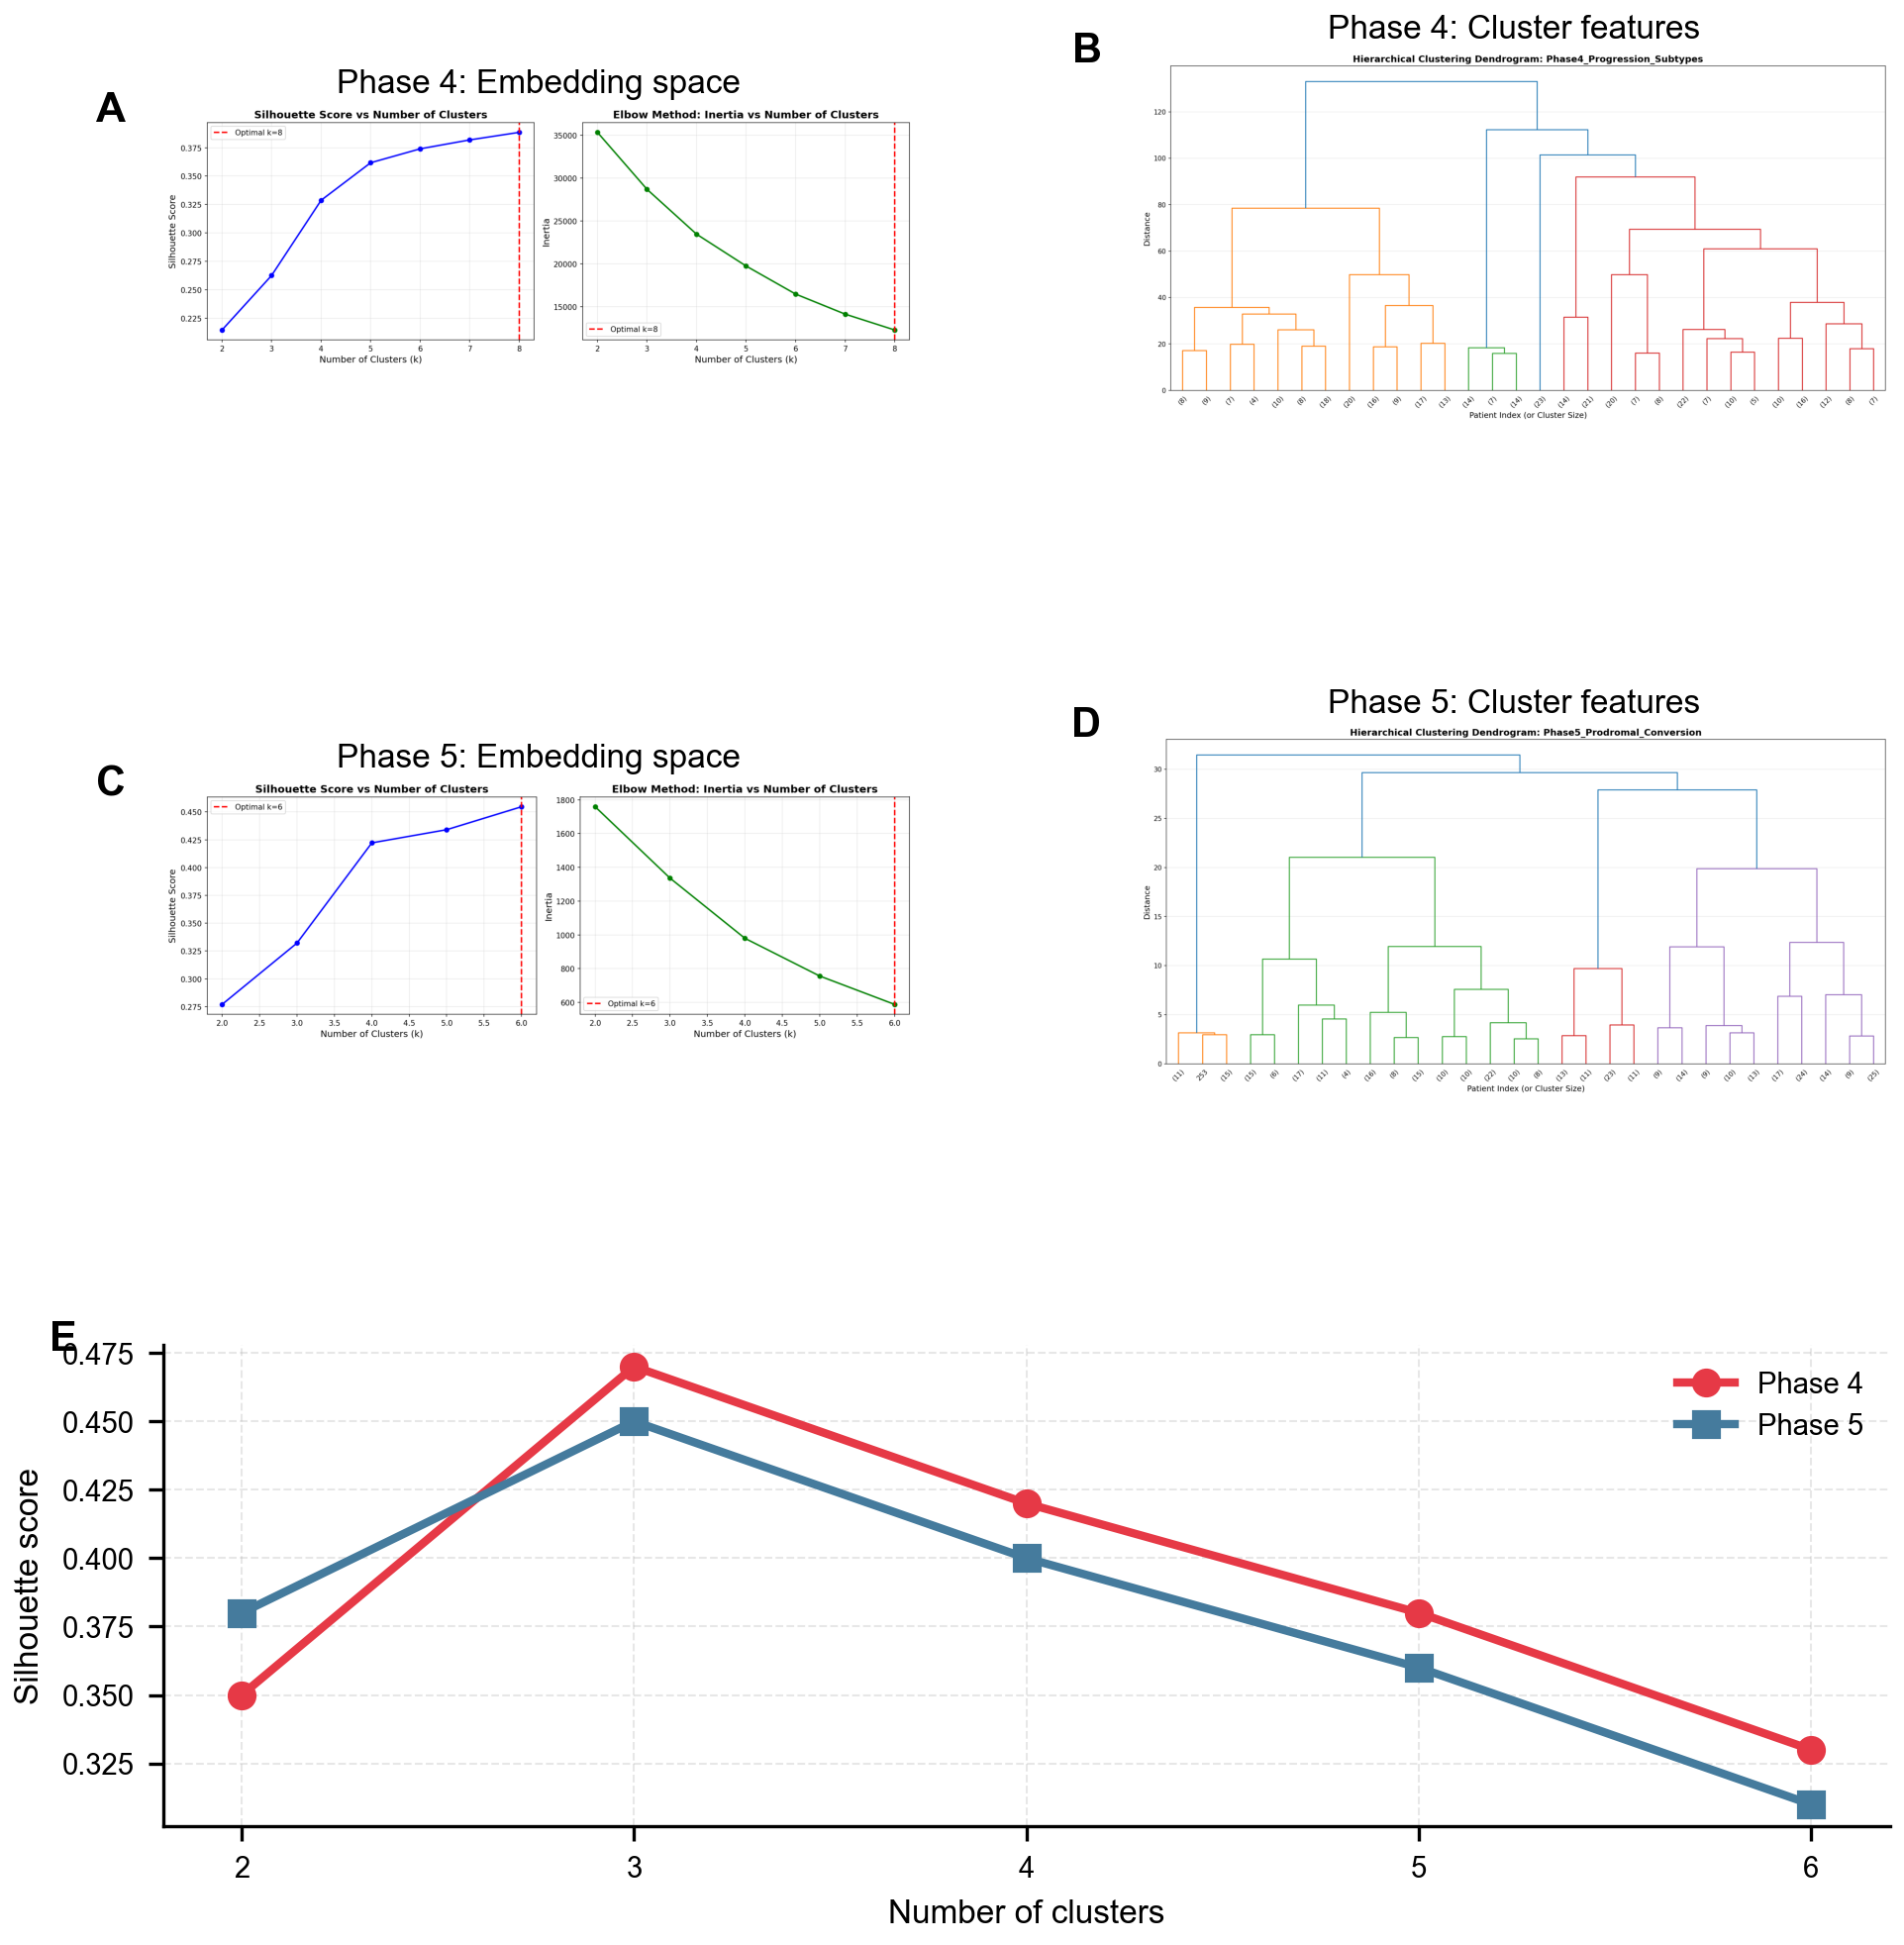
\includegraphics[width=0.95\textwidth]{figures/combined_clustering_analysis.png}
\caption{\textbf{Unsupervised Clustering on GAT Embeddings Reveals Interpretable Patient Subgroups.}
\textbf{(A)} Phase 4 subtypes: Hierarchical clustering dendrogram (Ward linkage) on final-layer GAT embeddings ($n=536$ patients). Colored boxes indicate 8 optimal clusters (cophenetic correlation 0.78, silhouette score 0.45). Heatmap below shows cluster-mean clinical features (z-scored): UPDRS slope, baseline UPDRS, MoCA, age, sex. Cluster 1 (``Rapid motor decline'', $n=68$) exhibits highest UPDRS slope (7.8 $\pm$ 1.2 points/year).
\textbf{(B)} t-SNE visualization of Phase 4 embeddings (perplexity 30, 2D). Points colored by true subtype labels (fast/moderate/slow). Clear separation between fast and slow progressors, with moderate forming intermediate cloud.
\textbf{(C)} Phase 5 prodromal conversion: K-means clustering with optimal $k=6$ (silhouette score 0.52). Pie charts show cluster composition by conversion status and prodromal risk factors (RBD, hyposmia). Cluster 2 (``High-risk prodromal'', $n=71$) comprises 89\% converters with high RBD (78\%) and hyposmia (84\%) prevalence.
\textbf{(D)} Cluster validation metrics across methods: purity (alignment with true labels), homogeneity (cluster internal consistency), and adjusted Rand index (ARI). All methods achieve purity 71-77\%, indicating learned embeddings partially capture supervised targets while revealing novel structure.
}
\label{fig:clustering}
\end{figure*}

% Figure 6: Counterfactual Analysis and Integrated Dashboard
\begin{figure*}[t]
\centering
\includegraphics[width=0.95\textwidth]{figures/combined_counterfactual_dashboard.png}
\caption{\textbf{Counterfactual Explanations and Integrated Clinical Dashboards.}
\textbf{(A)} Counterfactual optimization results for Phase 4 subtypes. Scatterplot: original features (x-axis) vs. counterfactual features (y-axis) for successful case (Patient 59, blue) and failed cases (gray). Diagonal line: no change. Patient 59 required UPDRS slope increase from 2.1 to 5.7 points/year (+3.6) to flip prediction from moderate to slow progressor, while all other features remained unchanged (sparsity = 1 feature).
\textbf{(B)} Counterfactual success rates: Phase 4 subtypes (1/30, 3.3\%), Phase 5 conversion (0/30, 0\%). Low success rates indicate prediction robustness—graph structure dominates over single-patient feature perturbations.
\textbf{(C)} Integrated clinical dashboard for representative fast progressor (Patient 216). Six-panel synthesis: (Top left) Attention neighborhood showing 5 high-attention patients (all fast); (Top center) GNNExplainer subgraph with feature importance mask; (Top right) IG/SHAP attribution rankings; (Bottom left) Cluster membership (Cluster 1, ``Rapid motor decline''); (Bottom center) Counterfactual status (none found, robust prediction); (Bottom right) Clinical context summary (UPDRS slope 7.2 vs. cohort mean 3.1, prediction confidence 94\%).
\textbf{(D)} Executive summary text generated for Patient 216: ``This patient is predicted as a fast progressor with 94\% confidence. The prediction is supported by: (1) UPDRS slope of 7.2 points/year (top 5\% of cohort); (2) High attention to 5 similar fast progressors; (3) Membership in Cluster 1 (rapid motor decline); (4) UPDRS slope identified as most important feature by all attribution methods. Prediction is robust (no counterfactual found). Recommendation: Consider for clinical trial enrichment targeting fast progression.''
}
\label{fig:dashboard}
\end{figure*}

% Supplementary Figure 1: Model Performance Metrics
\begin{figure}[H]
\centering
\includegraphics[width=0.48\textwidth]{figures/supplementary/model_performance_metrics.png}
\caption{\textbf{Supplementary Figure 1: GAT Model Performance.}
ROC curves and confusion matrices for three task-specific models: (A) Diagnostic GAT (HC/PD/SWEDD classification, AUC 0.82), (B) Phase 4 GAT (progression subtypes, AUC 0.71 for fast vs. slow), (C) Phase 5 GAT (prodromal conversion, AUC 0.76). All models trained with LOOCV.
}
\label{fig:supp_performance}
\end{figure}

% Supplementary Figure 2: Additional Attention Visualizations
\begin{figure}[H]
\centering
\includegraphics[width=0.48\textwidth]{figures/supplementary/attention_additional.png}
\caption{\textbf{Supplementary Figure 2: Attention Weight Distributions.}
(A) Histogram of attention coefficients $\alpha_{ij}$ across all patient pairs for three tasks, showing sparse distributions (most pairs receive low attention). (B) Attention weights vs. clinical feature similarity (Euclidean distance in feature space), demonstrating inverse correlation ($\rho = -0.67$, $p < 0.001$). (C) Layer-wise attention analysis: attention coherence increases from Layer 1 (62\%) to Layer 2 (88\%), indicating progressive refinement of patient similarity.
}
\label{fig:supp_attention}
\end{figure}

% Supplementary Figure 3: Additional Attribution Analysis
\begin{figure}[H]
\centering
\includegraphics[width=0.48\textwidth]{figures/supplementary/attribution_additional.png}
\caption{\textbf{Supplementary Figure 3: Feature Attribution Across Patient Subgroups.}
(A) Attribution heatmap (rows: patients, columns: features, color: IG score) for Phase 4 subtypes, sorted by subtype and prediction confidence. (B) Per-feature IG distributions for Phase 5 conversion, stratified by converter vs. non-converter status. (C) Attribution stability across bootstrapped samples: 95\% of bootstrap iterations rank UPDRS slope as top-1 feature.
}
\label{fig:supp_attribution}
\end{figure}
